\documentclass{article}
\usepackage[french]{babel}
\usepackage[utf8]{inputenc}
\usepackage{graphicx}
\usepackage{geometry}
\usepackage{subfig}
\usepackage{listings}
\usepackage{courier}

\title{Rapport Projet S5}
\author{Romain PIERRE, Méo DESBOIS-RENAUDIN}
\date{Janvier 2023}

\makeatletter
\let\mytitle\@title
\let\myauthor\@author
\let\mydate\@date
\makeatother

\begin{document}

\graphicspath{{tex/files/}}

\lstset{language=C, frame=single, basicstyle=\ttfamily, tabsize=4}

\begin{titlepage}
    \centering
    \vspace*{0.5 cm}
    
\includegraphics[width=3cm]{logo.jpg}\\[1.0 cm]
    \rule{\linewidth}{0.2 mm} \\[0.4 cm]
    \huge\textbf{\mytitle}\\
    \rule{\linewidth}{0.2 mm} \\[1.5 cm]  
    \LARGE\myauthor\\[2.0 cm]
    \large\textbf{\mydate}\\[2 cm]
    \begin{center}
        "MANSUBA"
    \end{center}

    \vspace{5cm}
    \begin{center}
    EI5PR103 - Projet d'algorithmique et de programmation
    \\Département Informatique
    \\S5 - Année 2022/2023
    \end{center}
 \end{titlepage}

\tableofcontents

\newpage
\section{Introduction}
Ce projet vise à réaliser divers algorithmes et structures de données, afin de faire jouer
à l'ordinateur des parties de jeux de plateau. Le code doit être fait de sorte à être modulable,
afin de faciliter l'ajout de fonctionnalité et la réalisation des divers modes de jeu.
\\\\
Ainsi, le plateau de jeu est représenté par une grille de positions en deux dimensions. La première dimension
est de taille WIDTH et est la largeur du plateau, la deuxième quant à elle est de taille HEIGHT et représente 
la hauteur du plateau, ainsi que le nombre de pièces de chaque joueur.
\\\\
Le plateau est donc de dimension $WORLD\_SIZE = WIDTH * HEIGHT$, chaque position est composée d'une couleur de joueur 
ou non, ainsi que d'un type de pièce ou non, selon la présence d'un joueur sur cette dernière.
\\\\
Chaque type de pièce a ses propres mouvements. De même, le type de plateau peut varier et ainsi, les voisins d'une 
position ne sont pas toujours les mêmes (exemples: grille classique (8 voisins), grille carrée(4 voisins), grille 
triangulaire (6 voisins)).

\newpage
\section{Architecture du projet}
\subsection{Dépendances}
Comme le montre la figure~\ref{depend}, nous avons décidé de séparer nos fonctionnalités en plusieurs fichiers, afin de gagner en clarté, logique et modularité. Ainsi, en plus du fichier
\textit{geometry} (qui régit toutes les constantes géométriques du problème), du fichier \textit{neighbors} (qui s'occupe des relations entre voisins),
et du fichier \textit{world} (qui génère le monde et ses accès, c'est-à-dire le plateau),  nous avons rajouté ces fichiers:
\\
\begin{itemize}
    \item \textit{play} qui contient les fonctionnalités de jeu.
    \item \textit{game} qui contient les règles du jeu et leur initialisation.
    \item \textit{set} qui contient la structure de gestion des pièces des joueurs et ses "méthodes".
    \item \textit{view} qui contient les fonctionnalités d'affichage.
\end{itemize}

\begin{figure}[h]
    \centering
    \subfloat{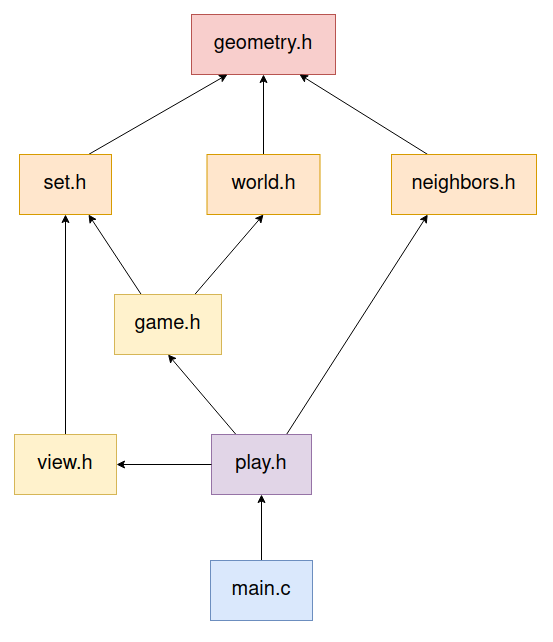
\includegraphics[width=0.4\textwidth]{graphe_dependances}}
    \caption{Graphe des dépendances}
    \label{depend}
\end{figure}

\subsection{Séparation des concepts, programmation modulaire}

L'intérêt premier de ce choix d'architecture est d'avoir un code modulaire. En effet, en regroupant les sous-problèmes en fichiers distincts,
il est plus facile de le maintenir ou de l'améliorer. Il suffit de respecter l'interface de base, et on peut ensuite travailler librement au sein même du fichier
sans altérer le reste du projet. De même, il n'est pas nécessaire d'avoir tous le projet en tête, et la simple connaissance du fichier en question est suffisante
pour travailler dessus.
\\\\
Ainsi, la programmation modulaire facilite la modification du code et limite les bugs qui pourraient se généraliser à l'ensemble du projet, en contenant l'information au sein d'un fichier.
Il est donc plus facile de se repérer, et de collaborer.

\newpage

\subsection{Début d'objectisation}

Lors de notre travail en groupe, nous avons dû créer des structures que l'on peut réutiliser dans le reste du code sans forcément en comprendre le fonctionnement intérieur.
Cela se voit particulièrement sur notre implémentation de \lstinline{set_t}.
Pour utiliser cette structure, en principe, il ne faut pas modifier les variables internes de la structure directement.
Pour la modifier, il faut utiliser des fonctions intermédiaires.
\\\\
On peut par exemple voir que nous avons donné un panel de fonctions intermédiaires pour modifier notre \lstinline{set_t} (listing \ref{lis:set}).
Elles permettent d'ajouter une position, d'en supprimer, d'effectuer des tests de présence et d'égalités, etc...
C'est un début d'\emph{encapsulation}.
Dans l'idéal, nous aurions aussi dû fournir des fonctions pour accéder aux variables internes de la structure, pour être plus rigoureux.
\\\\
Cependant, même si l'encapsulation n'est pas totalement respectée dans notre projet, nous avons quand même tiré beaucoup de bénéfices de cette structure.
Nous l'avons utilisé pour la majeure partie des fonctionnalités de notre projet et nous avons quand même pu effectuer des modifications internes sur celle-ci sans affecter le reste du projet.

\begin{lstlisting}[caption=set\_t, label=lis:set]
// struct representing a set of places
struct set_t {
  unsigned int size;
  unsigned int places[WORLD_SIZE];
};

// Select randomly a place in a set
unsigned int choose_random_place_in_set(struct set_t pieces);

// return union of a and b
struct set_t set_union(struct set_t a, struct set_t b);

// add p to s (with doublon gestion)
void add_place(struct set_t *s, unsigned int p);

// remove place p from set s 
void remove_place(struct set_t *s, unsigned int p);

// returns 1 if p is in the set
int is_in(struct set_t s, unsigned int p);

//test equality of 2 sets
int equal(struct set_t a, struct set_t b);
\end{lstlisting}

\label{set}



\newpage
\section{Fonctionnalités standards}
\subsection{Mouvements}
Un mouvement se décompose en deux étapes, le choix de la pièce qui va être jouée, puis le choix de sa nouvelle position.
\\\\
Ainsi on choisit aléatoirement une pièce dans le set de pièce active(voir section~\ref{set}). La pièce choisie ne doit pas être une pièce arrivée
chez l'adversaire (condition de victoire). Puis on liste les mouvements possibles selon le 
type de la pièce, et la relation en cours. Chaque type de pièce a donc sa propre fonction de listage de mouvements. Puis on choisit aléatoirement
un mouvement de la liste et on l'éxécute sur le monde, et dans les sets.
\\\\
À noter que le choix aléatoire d'un mouvement parmi la liste des mouvements possibles n'était vrai que dans un premier temps. Nous avons par 
la suite implémenté de nouvelles fonctions pour rendre ce choix plus intelligent et intéressant (voir section~\ref{sec:IA}).

\subsection{Relation}
Le projet nous amène à définir des relations entre les positions. Une relation est ici un ensemble de directions, ouvertes
ou fermées, qui autorisent ou non son déplacement dans cette dite direction (pour peu que le type de pièce l'autorise). Les relations
doivent être facilement accessibles et modifiables, car elles pourront changer au cours d'une même partie.
\\\\
Ainsi, nous avons choisi d'implémenter une variable globale "relation", sous la forme d'un tableau de 8 entiers. Chaque case représentant
une direction et valant 0 si la direction est fermée (le mouvement dans cette direction n'est pas possible), 1 sinon (le mouvement est possible
dans cette direction). La figure~\ref{carre} montre une représentation de la variable "relation" pour une grille carrée.

\begin{figure}[h]
    \centering
    \subfloat{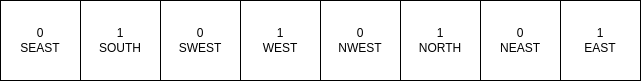
\includegraphics[width=0.8\textwidth]{relation.png}}
    \caption{État de la variable globale "relation" pour une grille carrée}
    \label{carre}
\end{figure}
Cette implémentation est donc très facile, car elle permet de modifier la relation en cours simplement en modifiant les valeurs des cases de relation.
Toutefois elle présente une limite, la relation doit être la même pour toutes les cases. Ainsi, nous ne pouvons pas par exemple faire de grille asymétrique.
Les grilles doivent nécessairement avoir un motif régulier qui se répète à chaque position.

\newpage
\subsection{Capture}
Dans notre projet, la capture s'active en modifiant le paramètre \lstinline{capture_activated} du struct \lstinline{game_t} régissant
les règles de la partie. La capture (si activée) est relativement simple. On autorise la pièce choisie pour le déplacement à, en plus des cases libres
et accessibles, se déplacer sur la première case rencontrée contenant une pièce adverse, dans une direction donnée.
\\\\
La seule contrainte est que l'on ne peut capturer une pièce arrivée sur nos positions de départ (condition de victoire), ou sur celle de l'adversaire (car impossibilité
de se libérer après, notre pièce étant arrivée et ne bougeant plus (voir détail section suivante \ref{liberation})).
\vspace{3cm}
\subsection{Libération}
\label{liberation}

La fonctionnalité de libération est quant à elle un peu plus complexe. Quand c'est son tour, le joueur va devoir choisir entre jouer un mouvement, ou
jouer une tentative de libération. S'il n'a pas de pièce capturée, il va automatiquement jouer un mouvement. Sinon, le choix entre mouvement et libération se
fera aléatoirement selon une probabilité p (fixé à 0.5). Si le mouvement est choisi, c'est un tour classique, sinon, la réussite de la libération 
se fera encore selon une probabilité q (là aussi fixé à 0.5).
\\\\
Si la libération réussie, il reste encore à ce que l'ancienne case de la pièce qui doit être libérée soit libre. En effet, une pièce capturée
ne peut revenir en jeu que sur sa case de capture. Si la case n'est pas libre, la libération échoue, sinon la pièce revient en jeu et le tour finit.
\\\\
Ces complications permettent de rendre la libération d'une pièce difficile, sans toutefois être impossible. Ainsi, la capture est un mécanisme
intéressant pour prendre l'avantage sur l'adversaire, sans toutefois lui être fatale.
\newpage
\section{Modes de jeu et implémentation}
\subsection{Gestion des paramètres de partie}
\label{gamet}
L'essentiel des paramètres de la partie est contenu dans la structure de données \lstinline{game_t} :

\begin{lstlisting}[caption=game\_t]
    struct game_t
    {
        struct world_t *w;
        struct set_t players_pieces[MAX_PLAYERS];
        struct set_captured_t captured_pieces[MAX_PLAYERS];
        enum color_t left_player_color;
        int rel;
        int change_rel;
        int capture_activated;
        enum board_type_t board_type;
    };
\end{lstlisting}

Voici les détails de sa composition :
\begin{itemize}
    \item \lstinline{struct world_t *w} :
    \\ pointeur sur le monde(représentant le plateau).
    \item \lstinline{struct set_t players_pieces[MAX_PLAYERS]} :
    \\ tableau de \lstinline{set_t} de taille \lstinline{MAX_PLAYERS} représentant les pièces actuellement
    en jeu des joueurs.
    \item \lstinline{struct set_captured_t captured_pieces[MAX_PLAYERS]} :
    \\ tableau de \lstinline{set_captured_t} de taille \lstinline{MAX_PLAYERS} représentant les pièces actuellement
    capturées des joueurs.
    \item \lstinline{enum color_t left_player_color} :
    \\ couleur du joueur qui joue à gauche.
    \item \lstinline{int rel} :
    \\ relation actuelle du plateau (classique, carré, triangulaire).
    \item \lstinline{int change_rel} :
    \\ indique si le changement de relation est autorisé ou non.
    \item \lstinline{int capture_activated} :
    \\ indique si la capture de pièce est autorisée ou non.
    \item \lstinline{enum board_type_t board_type} :
    \\ indique le mode de jeu de la partie (standard, dames chinoises, échecs).
\end{itemize}
\vspace{1cm}
L'intérêt de cette structure est qu'elle regroupe toutes les règles de la partie en cours en un seul endroit, ainsi on peut
facilement y avoir accès dans nos fonctions sans surcharger les paramètres. De plus on s'assure de la généralisation des modifications de règles en cours de partie (exemple du changement de type de relation/plateau tous les  $\sqrt{MAX\_TURN}$).
\subsection{Modes de jeu}
Ainsi, il nous a été facile de définir des types de partie spécifiques. Voici le détail des modes de jeu que nous avons implémentés :
\newline
\begin{itemize}
    \item Mode -1: Ce mode est utilisé pour figer une partie spécifique, indépendante de l'aléatoire, et ainsi permettre d'effectuer certains tests
    facilement (déplacements de pièces, capture, etc).
    \newline
    \item Mode 0 (défaut): Ce mode présente toutes les fonctionnalités de jeu (capture, libération, changements de relation, tous les types de pièces).
    \newline
    \item Mode 1: Mode de jeu des dames chinoises (Pas de capture, grille triangulaire, que des pions).
    \newline
    \item Mode 2: Mode de jeu des échecs (version adaptée aux objectifs du projet :  capture, libération, grille classique(8 voisins), première ligne de pièces des échecs (cavalier = éléphant), pas de fin de partie type échec).
\end{itemize}

\vspace{3cm}
\subsection{Intérêt des énumérations}
Les types de pièces et les couleurs des joueurs ont été codés dans des énumérations distinctes. Elles suivent globalement la même forme suivante :
\\
\begin{lstlisting}[caption=Exemple d'énumération]
    enum color_t {
        NO_COLOR  = 0,  
        BLACK     = 1,
        WHITE     = 2,
        MAX_COLOR = 3,
    };
\end{lstlisting}
L'intérêt, en plus d'assigner facilement un nom expressif à un entier, et que l'énumération centralise l'information. Ainsi il est facile de rajouter un joueur,
il suffit de rajouter une couleur et d'augmenter le champ \lstinline{MAX_COLOR} et la macro \lstinline{MAX_PLAYER} et de définir ses positions de départ.
De même pour rajouter une pièce, en implémentant sa fonction de mouvement et en l'incluant aux pièces de départ.
\\\\
L'utilisation des énumérations nous permet donc de ne pas avoir à modifier l'interface existante en rajoutant des éléments, mais seulement
d'implémenter leurs fonctionnalités.

\newpage
\section{Intelligence artificielle} 
\label{sec:IA}

Jusque-là, tous les choix que devaient faire les joueurs à chaque tour étaient déterminés aléatoirement parmi les possibilités dont ceux-ci disposaient. 
Au cours de notre projet, nous avons été amenés à devoir faire agir les joueurs de manière à avancer vers la victoire.
Cette partie pose des problèmes algorithmiques qui nous ont amenés à nous renseigner sur la théorie des graphes et la recherche de chemin.

\subsection{Gestion des distances}

L'objectif de cette section est de trouver les coups qui rapprochent le plus une pièce d'une position cible (les positions de départ du joueur opposé).
Pour cela, nous avons appris comment implémenter des techniques de parcours du plateau.
Plusieurs algorithmes se présentaient à nous :
\begin{itemize}
    \item Calcul des distances grâce aux index des positions
    \item Parcours en largeur
    \item Algorithme de Djikstra 
    \\
\end{itemize}

Le Calcul des distances grâce aux indexs des positions nous a paru la première solution évidente.
Voici un exemple simplifié de fonction que cette méthode aurait pu utiliser pour la grille carrée :

\begin{lstlisting}[caption=exemple de distance]
// retourne la distance entre A(ax, ay) et B(bx, by)
int distance(int ax, int ay, int bx, int by) 
{
    int distanceX = abs(ax - bx);
    int distanceY = abs(ay - by);
    return distanceX + distanceY;
}
\end{lstlisting}

Cependant, cette implémentation n'était pas \textbf{modulaire} ! En effet, elle nécéssite une fonction différente pour chaque configuration de relations du plateau.
Nous avons donc écarté cette solution et nous nous sommes concentrée sur les deux solutions suivantes.
\\\\
L'algorithme de \textbf{Djikstra} est un algorithme de recherche de plus court chemin utilisant une file triée, 
il marche sur tout type de graphe et est basé sur le \textbf{parcours en largeur}.
Il est très utile quand le graphe possède des arêtes à distances variables (dans notre graphe toutes les arêtes sont de même distance)
\\\\
Nous avons préféré ce dernier (\textbf{parcours en largeur}) à \textbf{Djikstra} car il est plus simple à implémenter et répond bien à nos besoins.
\\\\
Le \textbf{parcours en largeur}, comme son nom l'indique, parcourt le graphe en partant d'un sommet ou d'un ensemble de sommets.
\`{A} chaque itération, il explore les voisins directs (non déja éxplorés) des sommets ayant étés éxplorés à l'itération précédente.
Il s'arrête lorsque'une position cible est atteinte (en rouge sur la figure~\ref{bfs}).

\begin{figure}[h]
    \centering
    \subfloat[Itération 1]{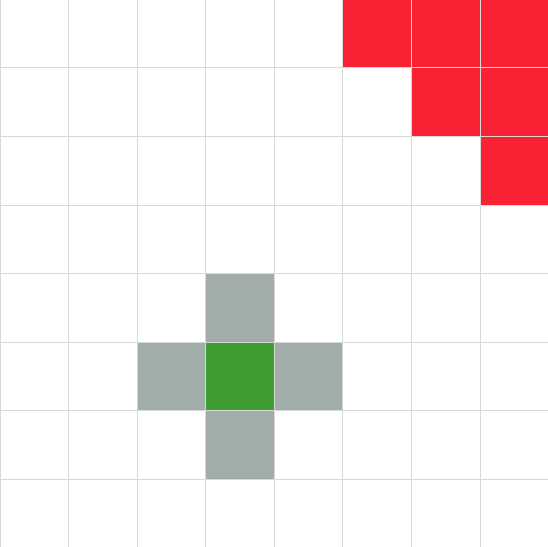
\includegraphics[width=0.3\textwidth]{bfs1.png}\label{fig:bfs1}}
    \hfill
    \subfloat[Itération 2]{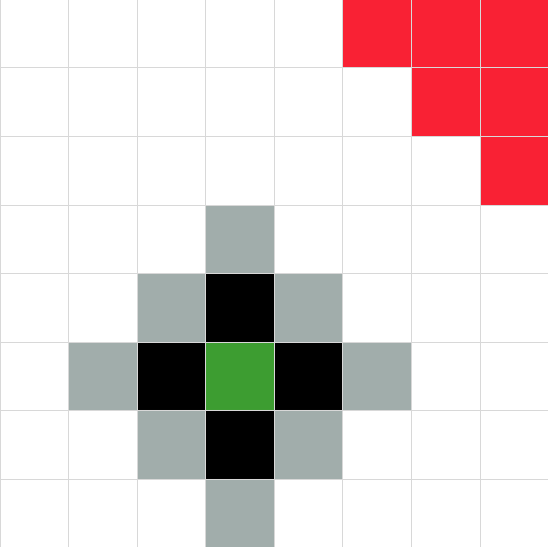
\includegraphics[width=0.3\textwidth]{bfs2.png}\label{fig:bfs2}}
    \hfill
    \subfloat[Itération 3]{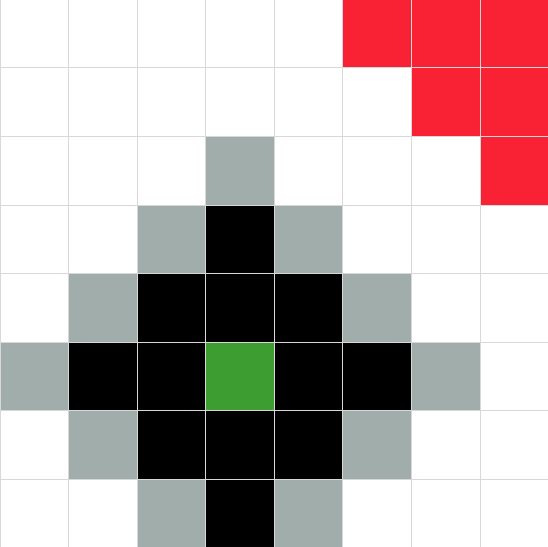
\includegraphics[width=0.3\textwidth]{bfs3.png}\label{fig:bfs3}}
    \caption{Exemple de \textbf{parcours en largeur} sur une grille carrée}
    \label{bfs}
\end{figure}

\subsection{Recherche du meilleur coup possible}

La méthode précédente a permis aux joueurs contrôlés par l'ordinateur d'atteindre les positions finales en beaucoup moins de tours qu'auparavant et on a même pu observer des victoires complexes.
Cependant, cette méthode présente des inconvénients :
\begin{itemize}
    \item Le chemin le plus rapide pour la pièce n'est pas forcément le plus proche
    \item Elle ne prend pas en compte si la route est barrée par une pièce ennemie
    \\
\end{itemize}

C'est pourquoi nous avons créé une version différente de notre parcours en largeur.
Le but de cette deuxième fonction est de simuler des mouvements de la pièce pour trouver quel est le chemin nécessitant \emph{le moins de tours} pour que la pièce atteigne sa cible.
\\\\
Dans cette version, à chaque itération, au lieu de visiter les voisins directs des sommets précédents, on visite les positions \emph{atteignables par un mouvement de la pièce} depuis les sommets précédents.
Ces positions atteignables sont déterminées par la fonction \lstinline{list_possible_moves_from_set()}.
\\\\
L'implémentation de cette fonction a été pour nous le plus gros défi algorithmique du projet. 
Mais cela nous a fait réfléchir aux algorithmes de recherche de chemin et nous a fait sortir de notre zone de confort. 
Nous n'avons sans doute pas trouvé la meilleure solution mais nous avons appris sur le chemin.

\newpage
\section{Affichage} 
\subsection{Options d'exécution et getopt}
Le projet ne nous amenait pas nécessairement à produire une interface graphique, mais celle-ci nous a paru primordiale pour faciliter
notamment les phases de debug, les tests, etc. De plus, il est plus agréable pour l'utilisateur de voir tous les détails de la partie.
\\\\L'affichage de la partie se fait donc à l'aide de l'option d'exécution -p (exemple: ./project -p). Nous avons implémenté nos options
d'exécution à l'aide de la librairie getopt. Cette librairie permet de récupérer des arguments de la ligne de commande et de faire des actions
en fonction d'eux. On peut donc changer les paramètres de notre partie directement depuis la console.
\\\\Sans l'option -p, l'utilisateur ne verra par défaut que la couleur de l'équipe gagnante (ou égalité, le cas échéant), ainsi que
le nombre de tours qu'a duré la partie. Avec l'option, l'utilisateur verra en plus pour chaque tour:
\begin{itemize}
    \item l'état du plateau avec les pièces en couleurs(couleurs des joueurs et vert pour la pièce qui a effectuée
    le dernier mouvement).
    \item le type de plateau (relation).
    \item le numéro du tour.
    \item les pièces actuellement capturées.
    \item s'il y a eu tentative de libération de pièce et si oui, si elle a réussi ou non.
\end{itemize}

\begin{figure}[h]
    \centering
    \subfloat[Tentavive de libération]{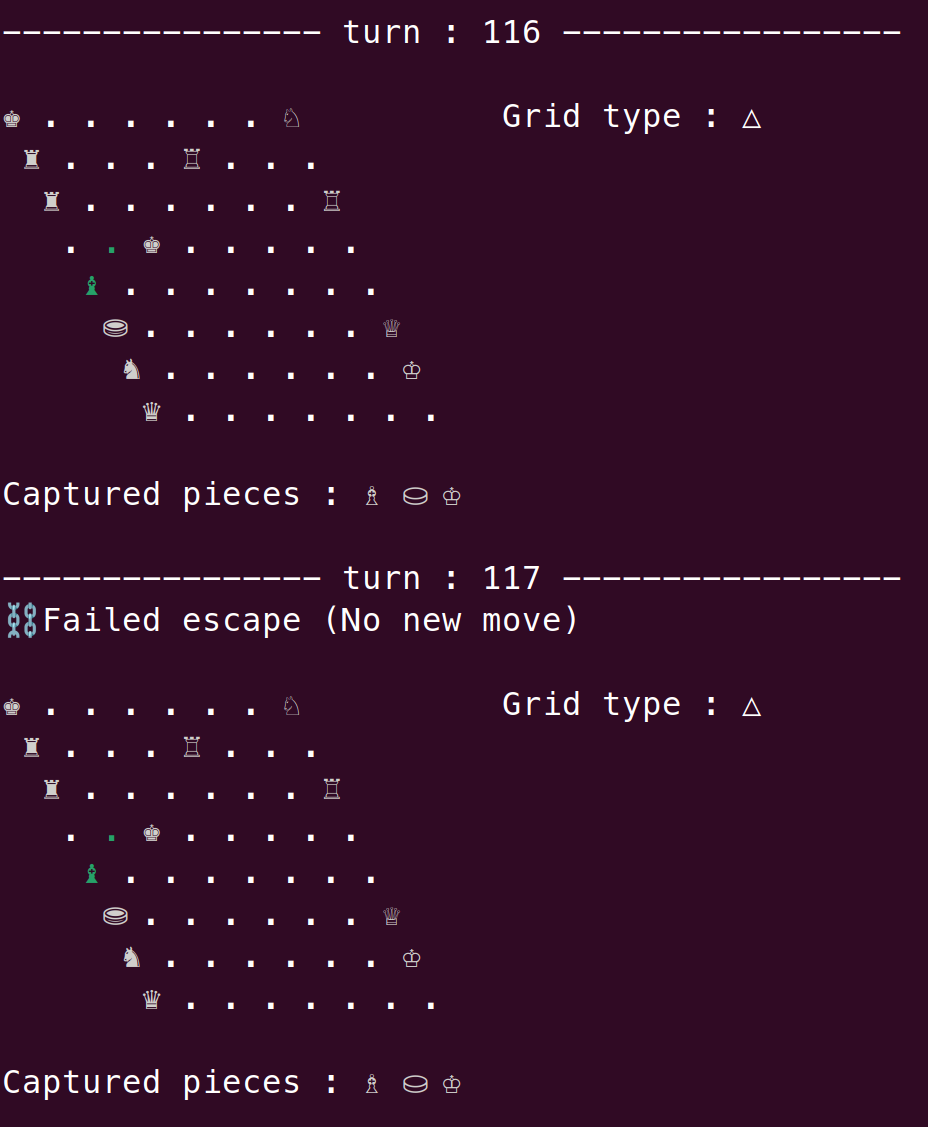
\includegraphics[width=0.28\textwidth]{exemplePrint2.png}\label{fig:sub1}}\hskip1ex
    \subfloat[Fin de partie]{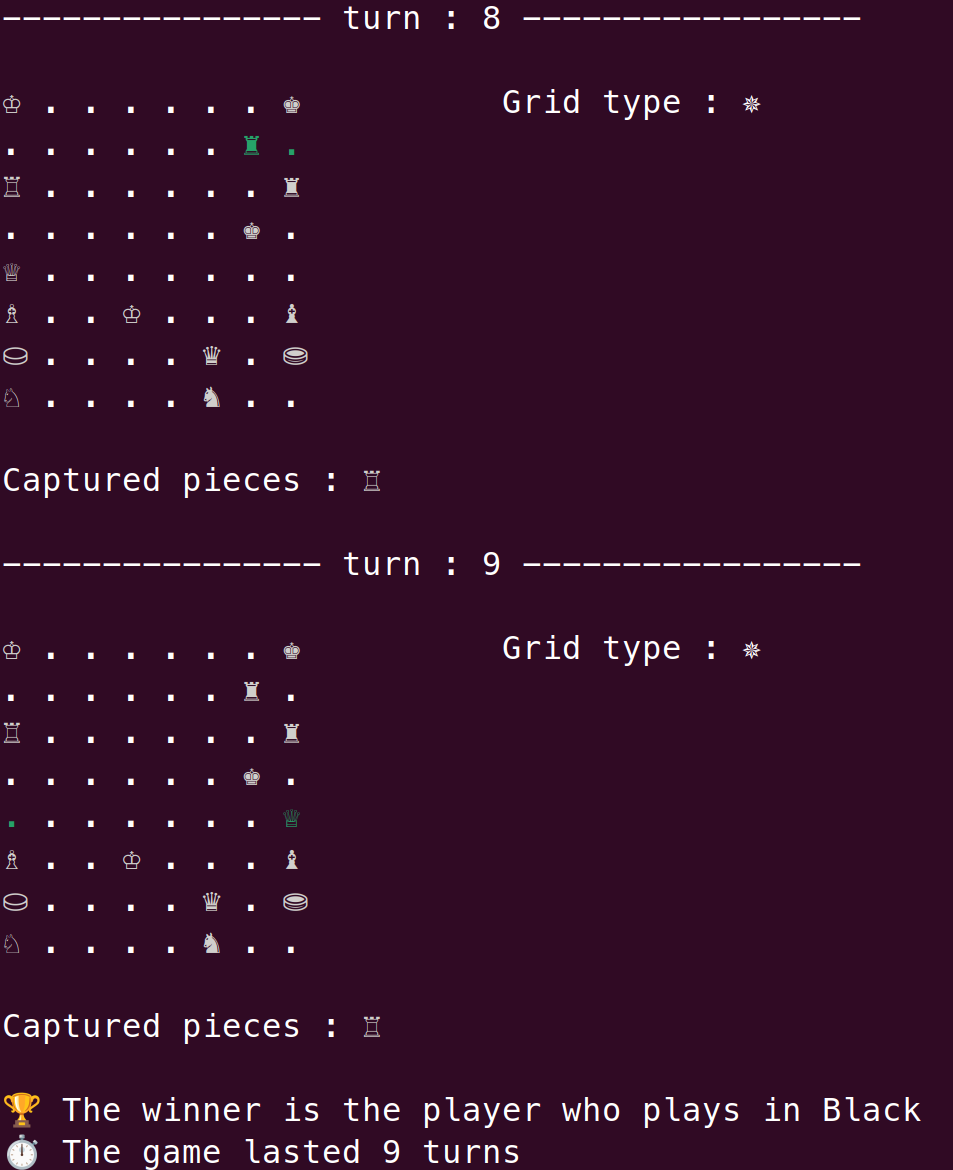
\includegraphics[width=0.28\textwidth]{exemplePrint1.png}\label{fig:sub2}}
    \caption{Exemples d'affichages avec l'option d'exécution -p}
    \label{print}
\end{figure}

La figure~\ref{print} montre des exemples d'affichages du programme dans le terminal en l'exécutant avec l'option -p. À noter
que l'affichage des pièces se fait au moyen du standard informatique : "Unicode".
\newline
\newline
Enfin, pour visualiser une partie comme si elle se déroulait en temps réel, nous avons décidé de rajouter une autre option d'exécution.
L'option "-d X" rajoute un délai de X microsecondes entre chaque coup et permet donc une simulation d'une partie en direct. Ainsi par exemple, pour voir une
partie avec une seconde entre chaque coup, l'utilisateur devra rentrer en commande "./project -p -d 1000000".

\newpage
\section{Performances} 

Durant notre projet, nous avons été amenés à faire des programmes complexes en temps et en espace.
Nous avons dû faire des compromis et choisir des solutions algorithmiques qui permettent de réduire au mieux ces complexités.

\subsection{Une structure fondamentale}

L'une des briques fondamentales de notre projet est la \lstinline{struct set_t}.
Cette structure représente un ensemble de positions sur notre plateau.
Il est très important que celle-ci soit optimisée \textbf{pour notre projet} car elle est utilisée dans une grande partie de nos fonctions dont celles qui sont appelées le plus de fois.
\\\\
Cette structure, pour notre projet, devait répondre à ces attentes :
\begin{itemize}
    \item Pas de doublons
    \item Test de présence rapide
    \item Accès à une position aléatoire rapide
    \item Test d'égalité rapide
    \item Complexité en espace au moins linéaire en fonction de \lstinline{WORLD_SIZE}
\end{itemize}

\begin{lstlisting}[caption=set\_t]
struct set_t {
    unsigned int size;
    unsigned int places[WORLD_SIZE];
};
\end{lstlisting}

L'implémentation que nous avons choisie est de représenter les positions sur les premières cases d'un tableau de taille \lstinline{WORLD_SIZE}. 
Ces positions restent \textbf{triées} à tout moment et on garde en mémoire le nombre de positions à l'intérieur.
\\\\
En prenant $N$ nombre de positions dans le set,
cette méthode nous permet d'obtenir les complexités en temps suivantes:
\begin{itemize}
    \item $O(log(N))$ pour tester la présence d'une position dans le set (dichotomie).
    \item $O(1)$ pour accéder à une position aléatoire du set.
    \item $O(N)$ pour le test d'égalité entre deux sets.
    \\
\end{itemize}
Cependant, elle est moins performante quand il faut modifier le set:
\begin{itemize}
    \item $O(N)$ pour ajouter un élément car il faut conserver l'ordre des positions.
    \item $O(N)$ pour supprimer un élément pour les mêmes raisons.
    \\
\end{itemize}

Au niveau de la complexité spatiale, toutes les fonctions de modification du \lstinline{set_t} ont des complexités \textbf{constantes}. 
Les fonctions d'accès et de tests ont des complexités au maximum \textbf{linéaires} en fonction de \lstinline{WORLD_SIZE}.
\\\\
De plus, les sets sont pour la grande majorité de taille inférieure à la racine carrée de \lstinline{WORLD_SIZE}.
Cela constitue le deuxième grand avantage de notre méthode, car celle-ci est complexe (temporellement) proportionnellement à la taille $N$ du set et non à \lstinline{WORLD_SIZE}.
\\\\
D'un côté la solution que nous avons choisi n'est pas forcément la meilleure, et elle contient des défauts. 
D'un autre côté, elle est stable et efficace sur les points importants de notre programme.
Ce projet nous a fait comprendre que chaque choix d'implémentation est un \textbf{compromis}.

\subsection{Des fonctionnalités coûteuses}

Certaines fonctions peuvent devenir très coûteuses en ressources rapidement si on augmente la taille du plateau ou le nombre de tours.
Regardons ces fonctions critiques et leurs limites.

\subsubsection{Déterminer le coup rapprochant le plus}

Comme nous l'avons dit dans la section~\ref{sec:IA}, nous avons utilisé un algorithme de parcours en largeur dans la fonction \lstinline{nearest_positions()} pour la recherche du coup rapprochant le plus la pièce des positions cibles.
Le parcours en largeur de base effectue au maximum une itération pour chaque arête du graphe que l'on explore.
Dans notre cas, il y a moins de $4 \times$\lstinline{WORLD_SIZE} arêtes.
De plus, pour chaque itération, on effectue une modification sur un set qui contient les prochains sommets à explorer.
Le set est au maximum de taille \lstinline{WORLD_SIZE}.
Comme la complexité temporelle de modification de set est linéaire en fonction de sa taille, Notre fonction \lstinline{nearest_positions()} a une complexité \textbf{quadratique} en fonction de \lstinline{WORLD_SIZE}.
\\\\
Calculons les limites de cette méthode :\\
Sachant que cette fonction est appelée à chaque tour et que le maximum de tour est $2 \times$\lstinline{WORLD_SIZE}.
En considérant que la machine tourne à 1 GHz et qu'on ne veut pas dépasser un temps d'exécution de 1 seconde.
Il faut effectuer moins d'un milliard d'instructions. Comme nous effectuons au maximum (\lstinline{WORLD_SIZE})$^3$ itérations.
Nous sommes limités à environ \lstinline{WORLD_SIZE} $< 1000$ \textit{i.e.} \lstinline{WIDTH}$\times$\lstinline{HEIGHT} $< 1000$.
\\\\
Cette méthode aurait pu être optimisée en utisant une autre structure de données que les \lstinline{set_t} mais elle nous a paru plus adaptée pour notre implémentation et système de relations.
\\
Cette fonction a une complexité temporelle conséquente, cependant, une autre fonction dans notre programme est encore plus gourmande en temps.

\subsubsection{Déterminer le coup pour atteindre l'objectif le plus rapidement}

La fonction qui permet de déterminer le coup amenant la pièce le plus rapidement sur la cible est \lstinline{choose_best_move()}.
Cette fonction est aussi basée sur un parcours en largeur, sauf que celle-ci appelle pour chaque position du monde la fonction \lstinline{list_possible_moves()}.
Cette dernière appelle une fonction spécifique à la \lstinline{sort_t} de la pièce étudiée.
Ces fonctions ont au maximum une complexité \textbf{quadratique} en fonction de \lstinline{WORLD_SIZE}.
En effet celles-ci font au maximum une modification sur des sets par position dans le monde.
\\
Comme cette fonction de complexité quadratique est appelée pour chaque position du monde dans \lstinline{choose_best_move()} et ce, à chaque tour, la complexité temporelle finale en ne considérant que cette fonction est $O(N^4)$ avec $N =$ \lstinline{WORLD_SIZE}.
\\\\
Finalement si on veut une exécution en temps raisonnable du programme, il faut respecter environ (\lstinline{WORLD_SIZE})$^4 <$ 1 000 000 000 \textit{i.e.} \lstinline{WORLD_SIZE} $< 177$.

\newpage
\section{Tests}
\subsection{Fonctionnement}
Pour effectuer nos tests, nous avons figé un type de monde spécifique pour ne plus dépendre de l'aléatoire des positions et des mouvements.
Puis chaque test effectue l'action spécifique qu'il doit vérifier. On récupère ensuite l'état du monde et des sets des joueurs, et on vérifie
que tout correspond bien à ce que l'on doit avoir. Si c'est le cas le test renvoie 1, sinon il renvoie 0. Cela nous sert ensuite pour l'affichage des résultats.

\vspace{2cm}
\subsection{Affichage des tests}
Les tests sont exécutés à l'aide de la commande "make test". L'exécutable est le même que le projet, à la différence que le main est remplacé par \lstinline{test.c}. Le programme exécute une batterie de tests et affiche en console si le test est passé ("OK"), ou pas ("ERROR"). La figure~\ref{test} donne un exemple de retour dans le terminal après la commande "make test".

\begin{figure}[h]
    \centering
    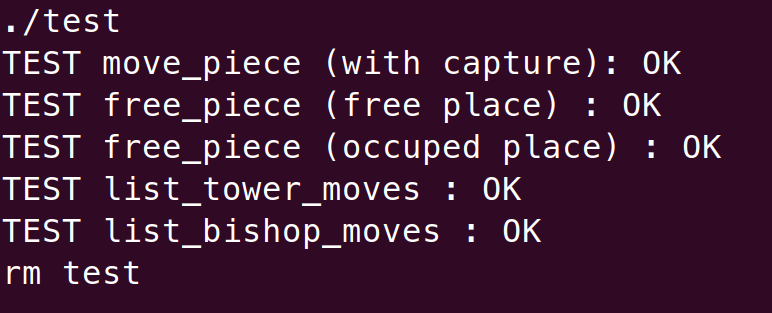
\includegraphics[width=5cm]{maketest.png}
    \caption{Retour console de la commande "make test"}
    \label{test}
\end{figure}

l'avantage de cette présentation des résultats est qu'en une commande, on peut facilement vérifier que l'ajout d'une nouvelle fonctionnalité n'a pas corrompu le fonctionnement des anciennes. Ainsi on peut garder facilement un projet fonctionnel, tout en y faisant des modifications.

\newpage
\section{Conclusion} 

Durant ce projet, nous avons été amenés à programmer en \emph{équipe}.
Nous avons dû nous répartir les tâches.
Nous avons dû utiliser et travailler avec des fonctionnalités codées par quelqu'un d'autre.
Cela n'a pas été facile dès le début, nous avions des visions différentes sur la structure du projet.
Et pour cause, nous avions tous les deux l'habitude de coder seul à notre manière.
Heureusement, au fil de ce module, nous avons réfléchi ensemble et avons appris à faire confiance à ce que l'autre codait.
\\\\
D'une part, nous devions continuellement changer notre code au rythme des achievements.
Nous avons vite compris qu'il n'allait pas être acceptable de retravailler tout notre travail à chaque nouvel achievement.
Nous avons donc dû commencer à apprendre à coder d'une manière permettant d'ajouter, de modifier ou de supprimer des fonctionnalités sans affecter le reste du projet.
Nous avons rendu notre code plus \emph{modulaire}.
\\\\
D'autre part, nous devions avoir un code clair, compréhensible et précis pour que notre camarade puisse comprendre notre code.
Pour cela, nous avons appris à éviter la \emph{duplication} du code, et à l'assembler en fonctions lisibles (c'est la \emph{factorisation}).
\\\\
Finalement, ce projet de programmation impérative nous a fait découvrir un nouveau langage de programmation.
Mais surtout il nous as fait comprendre comment coder en équipe, et comment rendre son code plus propre.
Nous avons pu comprendre les enjeux de la modularité dans les gros projets.
Ce projet nous as apporté un panel d'outils qui vont nous servir de fondation pour tous nos futurs projets.
Nous avons même pu commencer à avancer vers une "objectisation" du code avec \lstinline{set_t} et ses débuts d'encapsulation, nous amenant tout droit vers les prochains projets du semestre 6.

\end{document}
